\documentclass[a4paper]{article}
\usepackage[english]{babel}
\usepackage[utf8]{inputenc}
\usepackage{textcomp}
\usepackage{amsmath}
\usepackage{gensymb}
\usepackage{physics}
\usepackage{graphicx}
\usepackage[colorinlistoftodos]{todonotes}
\usepackage{xcolor}
\usepackage{array}
\usepackage{tabularx}
\usepackage{tikz}
\usepackage{framed}
\usepackage{xfrac}
\usepackage[most]{tcolorbox}
\usepackage{fix-cm}
\usepackage[margin=0.5in]{geometry}
\usetikzlibrary{quotes,angles}
\usetikzlibrary{decorations.pathreplacing}
\usetikzlibrary{calc}

\let\phi\varphi
\let\bf\textbf
\colorlet{shadecolor}{orange!15}
\def\centerarc[#1](#2)(#3:#4:#5){\draw[#1] ($(#2)+({#5*cos(#3)},{#5*sin(#3)})$) arc (#3:#4:#5)}
% Syntax: [draw options] (center) (initial angle:final angle:radius);

\title{Fixed-Axis Rotation}
\author{OpenStax University Physics Vol. 1}
\date{}

\begin{document}
\setcounter{section}{10}
\maketitle
\subsection{Rotational Variables}
\noindent\bf{Angular Velocity}
\vspace{2mm}\\
Uniform circular motion is motion in a circle at constant speed, although this is the simplest case of rotational motion, it is used here to introduce rotational variables.\par
The figure shows a particle moving in a circle. Its position vector from the origin of the circle to the particle sweeps out the angle $\theta$, which increases in the counterclockwise direction as the particle moves along its path. The angle $\theta$ is called the angular position of the particle. As the particle moves, it traces an arc length $s$.
\begin{center}
    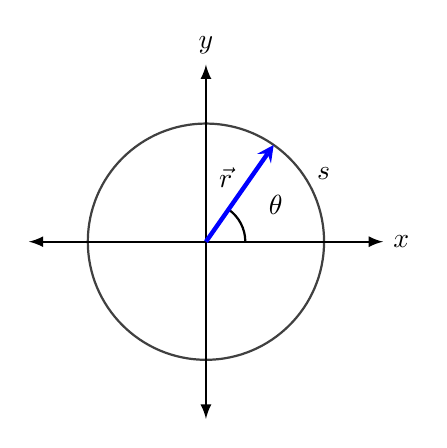
\begin{tikzpicture}[scale=1.5]
        %%% COORDINATES %%%
        \draw (0,0) coordinate (o);
        \draw ({cos(55)},{sin(55)}) coordinate (a);
        \draw ({cos(55)},0) coordinate (b);

        %%% AXES & CIRCLE %%%
        \draw[thick,draw=black!75] (0,0) circle (1);
        \draw[<->,thick,-latex] (0,0)--(1.5,0) node[right]{$x$};
        \draw[<->,thick,-latex] (0,0)--(0,1.5) node[above]{$y$};
        \draw[<->,thick,-latex] (0,0)--(-1.5,0);
        \draw[<->,thick,-latex] (0,0)--(0,-1.5);

        %%% POSITION VECTOR & ANGLE %%%
        \draw pic["$\theta$",draw=black,thick,-,angle eccentricity=2,angle radius=0.5cm]{angle=b--o--a};
        \draw[->,ultra thick,draw=blue,-stealth] (0,0)--node[left,xshift=0.5mm,yshift=2mm]{$\vec{r}$}({cos(55)},{sin(55)});

        \centerarc[red,very thick](0,0)(0:55:1);
        \node at ({1.15*cos(30)},{1.15*sin(30)}){$s$};
    \end{tikzpicture}
\end{center}
The angle is related to the radius of the circle and the arc length by 
\begin{equation}
    \theta = \frac{s}{r}
\end{equation}
The angle $\theta$, the angular position of the particle moving along its path has units of radians (rad). As the particle moves along its circular path, its angular position changes and it undergoes angular displacements $\Delta\theta$.\par\vspace{1mm}
\noindent We can assign vectors to the quantities in equation 1, the angle $\vec{\theta}$ is a vector out of the page. The angular position vector $\vec{r}$ and the arc length vector $\vec{s}$ both lie in the plane of the page, they are related by:
\begin{equation}
    \vec{s} = \vec{\theta} \times \vec{r}
\end{equation}
The arc length is the cross product of the angle vector and the position vector
\begin{center}
    \begin{tikzpicture}[scale=2]
        \draw[->,-latex] (0,0)--(1,0) node[right]{$y$};
        \draw[->,-latex] (0,0)--node[right]{$\vec{\theta}$} (0,1) node[above]{$z$};
        \draw[->,-latex] (0,0)--(-{cos(45)},-{sin(45)}) node[left]{$x$};

        \draw[->,very thick,-stealth] (0,0)--(0,0.75);
        \draw[->,very thick,-stealth] (0,0)--node[below,xshift=-2mm,yshift=0.5mm]{$\vec{r}$}({0.7*cos(65)},{-0.7*cos(65)});
        \draw[->,very thick,-stealth,draw=red] ({0.7*cos(65)},{-0.7*cos(65)})--node[right,yshift=-1mm,xshift=-0.5mm]{$\vec{s}$}({0.7*cos(65) + 0.28},{-0.7*cos(65) + 0.28});
    \end{tikzpicture}
\end{center}
The magnitude of the angular velocity, denoted by $\omega$, is the time rate of change of the angle $\theta$ as the particle moves in a circular path. The instantaneous angular velocity, defined as the limit as $\Delta t \to 0$ of the average angular velocity $\bar{\omega} = \frac{\Delta\theta}{\Delta t}$
\begin{equation}
    \omega = \lim\limits_{\Delta t \to 0}\frac{\Delta\theta}{\Delta t} = \frac{d\theta}{dt}
\end{equation}
Where $\theta$ is the angle of rotation. The units of angular velocity are radians per second (rad\;s$^{-1}$). Angular velocity can also be referred to as the rotation rate in radians per second. In many cases, rotation rate is given in revolutions/s or cycles/s, to find angular velocity, multiply revolutions/s by $2\pi$ (since there are $2\pi$ radians per revolution). Since a positive angle in a circle is counterclockwise, we take counterclockwise rotations as being positive and clockwise rotations as negative.

\end{document}